\documentclass{article}
\usepackage[utf8]{inputenc}
\usepackage[left=3cm, right=3cm, top=2cm]{geometry}
\title{Collisions: Non-linearities without the use of iterative solvers}
\author{Silvin Willemsen}
\date{April 2019}

\usepackage{natbib}
\usepackage{graphicx}
\usepackage{appendix}
\usepackage{amsmath}
\usepackage{amsfonts}
\usepackage{amssymb}
\usepackage{cases}
\usepackage{xcolor}
\usepackage{mathrsfs} 

\def\SBcomment[#1]{\textcolor{red}{#1}}
\def\SWcomment[#1]{\textcolor{blue}{#1}}

\begin{document}

\ifpdf % used graphic file format for pdflatex
  \DeclareGraphicsExtensions{.png,.jpg,.pdf,.eps} 
\else  % used graphic file format for latex
  \DeclareGraphicsExtensions{.eps}
\fi

\maketitle

\section{Introduction}
This document shows several examples of non-linearities in physical modelling based on a method recently published by Michele Ducceschi in \cite{Ducceschi2019}.

%Energy analysis proves to be a handy tool for verifying whether the devised system is stable or not.

\section{Preabmble: Mass-barrier collision}
The simplest collision case is a mass colliding with a rigid barrier. Imagine a mass at location $u = u(t)$ colliding with a barrier at location $b$. If the barrier is placed above\footnote{When talking about an element being `above' or `below' another in this context, what is meant is a more positive or negative displacement, i.e., a mass with a displacement of 0.01 will be `above' a barrier with a displacement of -0.05. Along these lines, a positive force acting on an element will accelerate it upwards and a negative force will accelerate it downwards.} the mass, the force it exerts on the mass will be negative and its system would be described as
\begin{equation}\label{eq:massBarrier}
    Mu_{tt} = -K[\eta]_+^\alpha,
\end{equation}
with mass $M$ (in kg), collision stiffness $K \geq 0$ (in N/m \SWcomment[???]) and non-linearity $\alpha \geq 1$ and $\eta = u - b$ describes the relative displacement between the two colliding bodies (in m).
\begin{equation}\label{eq:etaPlus}
    [\eta]_+ = \frac{\eta + |\eta|}{2}
\end{equation}
describes the positive part of $\eta$ (see Figure \ref{fig:eta}). This can be interpreted as that $\eta$ will only be non-zero when the two colliding bodies are in contact.

\begin{figure}[h]
\centerline{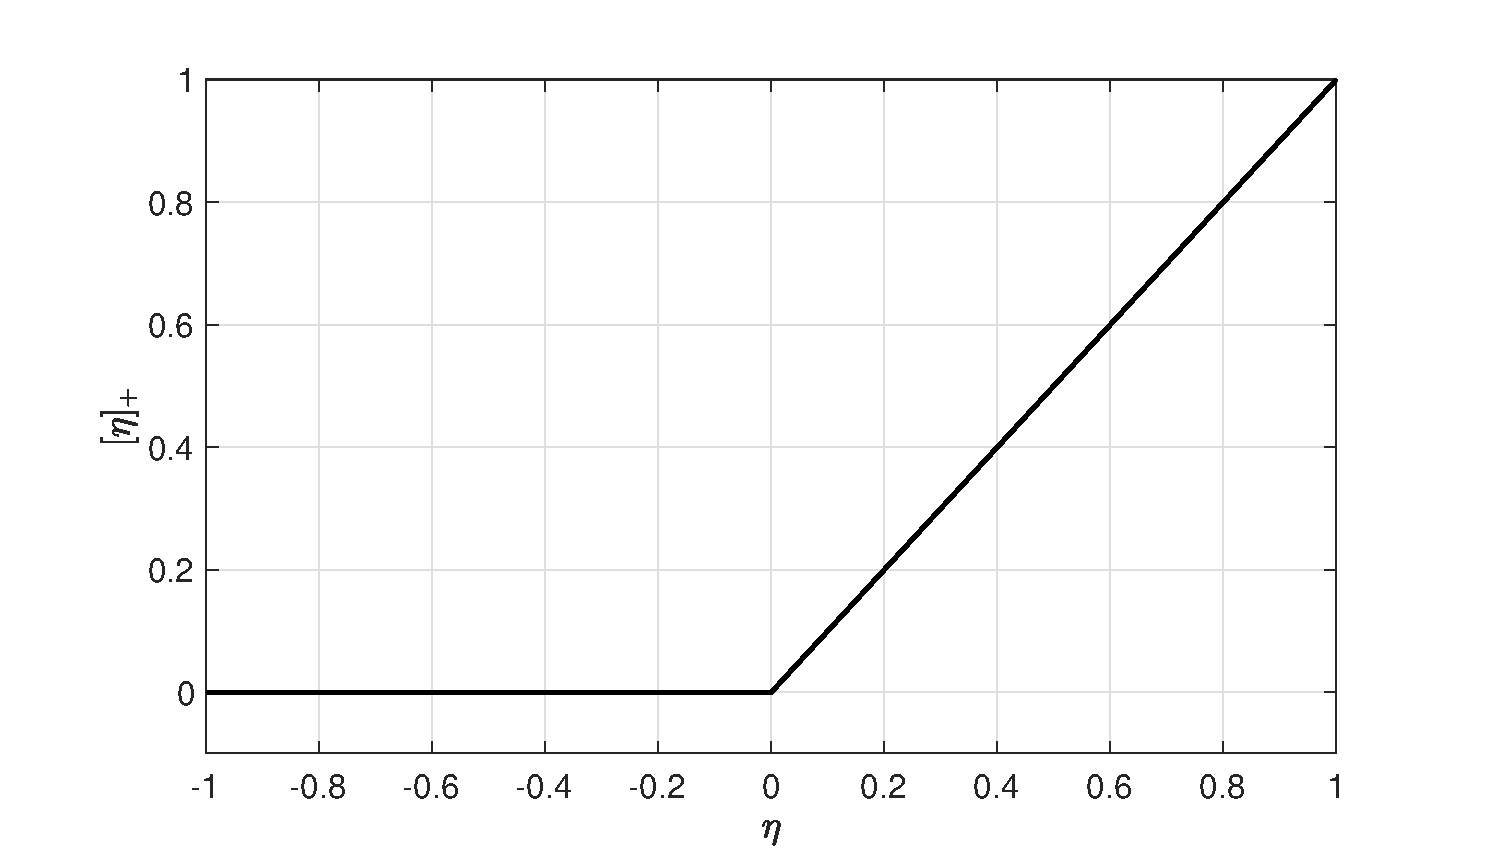
\includegraphics[width=0.6\columnwidth]{eta.eps}}
\caption{\label{fig:eta}{A plot of $[\eta]_+$.}}
\end{figure}

\noindent The second term can be rewritten to 
\begin{equation}\label{eq:derivPotential}
    \phi'(\eta) = \frac{d\phi(\eta)}{d\eta}\overset{\text{chain rule}}{\xrightarrow{\hspace*{1.4cm}}}  \frac{d\phi}{dt}\frac{dt}{d\eta} = \frac{\left(\frac{d\phi}{dt}\right)}{\left(\frac{d\eta}{dt}\right)}=\frac{\dot{\phi}(\eta)}{\dot{\eta}} =  K[\eta]_+^\alpha
\end{equation}
where
\begin{equation}\label{eq:potential}
    \phi(\eta) = \frac{K}{\alpha+1}[\eta]_+^{\alpha + 1}\ ,
\end{equation}
describes the potential energy of the system. Equation \eqref{eq:massBarrier} can then be rewritten to
\begin{equation}
    Mu_{tt} = -\phi'(\eta).
\end{equation}
According to Ducceschi in \cite{Ducceschi2019}, this potential has been used before in the literature, but when discretised, results in an implicit system for which an iterative solver (such as Newton-Raphson's method) must be employed. In his work, he proposes to rewrite the potential in Eq. \eqref{eq:derivPotential} as
\begin{equation}
    \psi\psi' \quad \text{where} \quad \psi = \sqrt{2\phi} \quad \text{and} \quad \psi' = \frac{\dot{\psi}}{\dot{\eta}}\ ,
\end{equation}
yielding
\begin{equation}\label{eq:massBarrierPsi}
    Mu_{tt}=-\psi\psi'.
\end{equation}
See Appendix \ref{app:phiPsiProof} for a proof that $\phi'$ is equivalent to $\psi\psi'$.
\subsection{Discrete time}
For the discrete time definition of $\psi'$ we can use 
\begin{equation}
    g^n = \frac{\delta_{t+}\psi^{n-1/2}}{\delta_{t\cdot}\eta^n},
\end{equation}
where $\psi$ at interleaved grid point $n-1/2$ is defined as
\begin{equation}
    \psi^{n-1/2} = \mu_{t-}\psi^n,
\end{equation} 
and is proven useful as \SWcomment[it requires less memory...] Equation \eqref{eq:massBarrierPsi} can then be discretised to the following system.\footnote{It is important to realise whether the mass is placed above or below the barrier as this will affect the following two things in \eqref{eq:massBarrierSystem}:
\begin{enumerate}
    \item The direction of the force (the sign of the term right-hand side in \eqref{eq:massBarrier1}): if the barrier is placed above the mass this will exert a downwards (negative) force on the mass, when below, the opposite applies. Of course, the sign used here is determined by the system described in \eqref{eq:massBarrier} where the force-term is negative.
    \item The definition of eta (what is subtracted from what?): imagine that the collision happens when $\eta$ is positive, so when the barrier is placed above the mass, $u^n-b$ will be positive on collision. Remember: $\eta$ is defined as the element above subtracted from the element below.
\end{enumerate}}
% \begin{equation}
% \begin{numcases}
%     $Mu_{tt} $&$= -\big(\mu_{t+}\psi^{n-1/2}\big)g^n$ \\
%     $\delta_{t+}\psi^{n-1/2} $& $=  g^n\delta_{t\cdot}\eta^n\ $,
% \end{numcases}
% % \end{equation}
\begin{subequations}\label{eq:massBarrierSystem}
\begin{numcases}{}
    M\delta_{tt}u^n & $= -\big(\mu_{t+}\psi^{n-1/2}\big)g^n$ \label{eq:massBarrier1} \\
   \delta_{t+}\psi^{n-1/2} &= $g^n\delta_{t\cdot}\eta^n$ \label{eq:massBarrier2} \\ 
   \eta^n &$= u^n - b$ \label{eq:etaMassBarrier}
\end{numcases}
\end{subequations}
\subsection{Implementation}
\subsubsection*{Step 1: Calculate $g^n$}
The first step is to calculate $g^n$ using its analytic derivative
\begin{equation}
    g^n = \psi'\bigg\rvert_{\eta=\eta^n} = \frac{\phi'}{\sqrt{2\phi}}\bigg\rvert_{\eta=\eta^n}
\end{equation}
which, using \eqref{eq:derivPotential} and \eqref{eq:potential}, can conveniently be rewritten to
\begin{equation}\label{eq:gn}
    g^n = \frac{K[\eta^n]_+^\alpha}{\sqrt{\frac{2K}{\alpha+1}[\eta^n]_+^{\alpha+1}}}=K\sqrt{\frac{\alpha+1}{2K}}[\eta^n]_+^\alpha[\eta^n]_+^{\frac{-(\alpha+1)}{2}}=\sqrt{\frac{K(\alpha+1)}{2}}[\eta^n]_+^{\frac{\alpha-1}{2}}\ .
\end{equation}
\subsubsection*{Step 2: Substitution of identity for $\mu_{t+}\psi^{n-1/2}$}
Using the following identity
\begin{equation}
    \mu_{t+}\psi^{n-1/2} = \frac{k}{2}\delta_{t+}\psi^{n-1/2} + \psi^{n-1/2},
\end{equation}
inserting \eqref{eq:massBarrier2} into this 
\begin{equation}\nonumber
    \mu_{t+}\psi^{n-1/2} = \frac{k}{2}g^n\delta_{t\cdot}\eta^n + \psi^{n-1/2},
\end{equation}
and inserting this into \eqref{eq:massBarrier1} yields
\begin{equation}\label{eq:substitutionFDS}
    M\delta_{tt}u^n = -\Big(\frac{k}{2}g^n\delta_{t\cdot}\eta^n + \psi^{n-1/2}\Big)g^n\ .
\end{equation}
\subsubsection*{Step 3: Solving the system for $u^{n+1}$}
As in this case, the position of barrier $b$ is static, the following is true:
\begin{equation}\label{eq:derEtaEqDerU}
    \frac{d\eta}{dt} = \frac{d}{dt}\Big(u - b\Big)\Rightarrow \delta_{t\cdot}\eta^n = \delta_{t\cdot}u^n,
\end{equation}
i.e., the time derivative of $\eta$ equals the time derivative of $u$.\footnote{Note that if the barrier was placed underneath the mass, making \eqref{eq:etaMassBarrier} $\eta^n = b-u^n$, this would result in $\delta_{t_\cdot}\eta^n = -\delta_{t\cdot}u^n$.} Now we can solve \eqref{eq:substitutionFDS} explicitly as $u^{n+1}$ is the only unknown
\begin{equation}
    \bigg(\frac{M}{k^2} + \frac{(g^n)^2}{4}\bigg)u^{n+1} = \frac{M}{k^2}(2u^n-u^{n-1})+\frac{(g^n)^2}{4}u^{n-1}-\psi^{n-1/2}g^n\ ,
\end{equation}
and can be solved by a simple division. 
\subsubsection*{Step 4: Calculate $\eta^{n+1}$ and $\phi^{n+1/2}$} From this, $\eta^{n+1}$ can be calculated using \eqref{eq:etaMassBarrier}:
\begin{equation}\label{eq:etaNPlus1}
    \eta^{n+1} = u^{n+1}-b,
\end{equation}
and can be used to calculate $\psi^{n+1/2}$ by expanding and rewriting \eqref{eq:massBarrier2} to
\begin{equation}\label{eq:psiNPlusHalf}
    \psi^{n+1/2} = \psi^{n-1/2} + \frac{\eta^{n+1} - \eta^{n-1}}{2}.
\end{equation}

\section{Mass-spring - Rigid barrier collision}
If the mass described in the previous section (Eq. \eqref{eq:massBarrierPsi}) is given a restoring force, the following equation emerges
\begin{equation}\label{eq:massSpringBarrier}
    Mu_{tt} = -M\omega_0^2u - \psi\psi'.
\end{equation}
where $\omega_0 = 2\pi f_0$ is the angular frequency of the mass-spring system (in s$^{-1}$) with fundamental frequency $f_0$ (in Hz). This system can be discretised to the following system (similar to \eqref{eq:massBarrierSystem})

\begin{subnumcases}{}
    M\delta_{tt}u^n &$= -M\omega_0^2u^n - \big(\mu_{t+}\psi^{n-1/2}\big)\,g^n,$\\
    \delta_{t+}\psi^{n-1/2}& $=g^n\delta_{t\cdot}\eta^n$\\
    \eta^n &$= u^n - b$
\end{subnumcases}
where $g^n$ is again computed according to \eqref{eq:gn}. The system can, similarly to the one in the previous section, be discretised to
\begin{equation}
    \bigg(\frac{M}{k^2} + \frac{(g^n)^2}{4}\bigg)u^{n+1} = \frac{M}{k^2}(2u^n-u^{n-1})-M\omega_0^2u^n +\frac{(g^n)^2}{4}u^{n-1}-\psi^{n-1/2}g^n\ ,
\end{equation}
after which $\eta^{n+1}$ using \eqref{eq:etaNPlus1} and $\psi^{n+1/2}$ using \eqref{eq:psiNPlusHalf} can be calculated. 

\section{Mass-spring - Mass-spring Collision}
The initial idea for this implementation was to make the barrier in the previous section able to move sinusoidally. However, as the barrier would be unaffected by the mass, the energy balance would be incorrect. Imagine a baseball bat hitting a ping-pong ball. Even though the bat would not seem to be affected by the ping-pong ball, it will as some energy of the ball will be transferred into the bat. To model this behaviour, we can implement two colliding masses, one of which has a very high mass relative to the other, and to make it more interesting, we can add a restoring force to both. Assuming a mass with displacement $u = u(t)$ to be placed above a mass with displacement $w = w(t)$, the (continuous) system will look like this 

\begin{subnumcases}{}
    M_1u_{tt} &$=-M_1\omega_1^2u+\psi\psi'$\\
    M_2w_{tt} &$=-M_2\omega_2^2w-\psi\psi'$
\end{subnumcases}
which, when discretised yields
\begin{subequations}\label{eq:mSmSDisc}
\begin{numcases}{}
    M_1\delta_{tt}u^n &$= -M_1\omega_1u^n+\Big(\mu_{t+}\psi^{n-1/2}\Big)g^n$\label{eq:massMass1}\\
    M_2\delta_{tt}w^n &$= -M_2\omega_2w^n-\Big(\mu_{t+}\psi^{n-1/2}\Big)g^n$\label{eq:massMass2}\\
    \delta_{t+}\psi^{n-1/2}& $=g^n\delta_{t\cdot}\eta^n$\\
    \eta^n &$= w^n - u^n$\label{eq:etaMSMS}
\end{numcases}
\end{subequations}
Note that the term denoting the collision will have a positive effect on $u$ and a negative effect on $w$ as $u$ is placed above $w$.

As we are now working with two moving objects colliding, \eqref{eq:derEtaEqDerU} is not valid anymore. The main challenge here, is to solve the system for two unknowns: $u^{n+1}$ and $w^{n+1}$. Rewriting \eqref{eq:massMass1} and \eqref{eq:massMass2} in terms of these two unknowns yields

\begin{align}
    \mathbf{A}
    \begin{bmatrix}
        u^{n+1}\\
        w^{n+1}
    \end{bmatrix}
    = 
    \mathbf{v} \quad\Rightarrow \quad 
    \begin{bmatrix}
        u^{n+1}\\
        w^{n+1}
    \end{bmatrix} = \mathbf{A}^{-1}\mathbf{v}
\end{align}
where 
\begin{equation}
    \mathbf{A} = \begin{bmatrix}
        \frac{M_1}{k^2}+\frac{(g^n)^2}{4} & -\frac{(g^n)^2}{4} \\
        -\frac{(g^n)^2}{4} & \frac{M_2}{k^2} + \frac{(g^n)^2}{4}
    \end{bmatrix}
    \quad\text{and}\quad\mathbf{v} =
    \begin{bmatrix}
        \frac{M_1}{k^2}(2u^n-u^{n-1})-M_1\omega_1u^n-\frac{(g^n)^2}{4}\eta^{n-1}+\psi^{n-1/2}g^n\\
        \frac{M_2}{k^2}(2w^n-w^{n-1})-M_2\omega_2w^n+\frac{(g^n)^2}{4}\eta^{n-1}-\psi^{n-1/2}g^n
    \end{bmatrix}\nonumber
\end{equation}
See Appendix \ref{app:massMassDeriv} for the deriviation of this. The relative displacement $\eta^{n+1}$ can then be calculated using \eqref{eq:etaMSMS}.

\section{String - String Collision}\label{sec:stringString}
Moving to a string - string collision, we can define states $u = u(x,t)$ and $w = w(x,t)$ which are now distributed or defined over spatial coordinate $0\leq x\leq L$ where $L$ is the length of the repective string. Using the definitions of the stiff string defined in, fx., \cite{Bilbao2009}, the continuous system is defined as

\begin{subequations}
    \begin{numcases}{}
        \rho_1 A_1u_{tt} &$= T_1u_{xx}-E_1I_1u_{xxxx}+\psi\psi'$\\
        \rho_2 A_2w_{tt} &$= T_2w_{xx}-E_2I_2w_{xxxx}-\psi\psi'$
    \end{numcases}
\end{subequations}
with material density $\rho$ (in kg$\cdot$m$^{-3}$), cross-sectional area $A=\pi r^2$ (in m$^2$) with radius $r$ (in m), tension $T$ (in N), Young's modulus E (in Pa) and area moment of inertia $I = \pi r^4/4$ (in m$^4$) of string $1$ with displacement $u$ and string $2$ with displacement $w$ respectively. When discretising this, $x=lh$ for grid point $l\in[0, ..., N]$ and grid spacing $h$, yields
\begin{subequations}
\begin{numcases}{}
    \rho_1A_1\delta_{tt}u_l^n &$= T_1\delta_{xx}u_l^n-E_1I_1\delta_{xxxx}u^n_l+\Big(\mu_{t+}\psi^{n-1/2}_l\Big)\,g^n_l$\\
     \rho_2A_2\delta_{tt}w_l^n &$= T_2\delta_{xx}w_l^n-E_2I_2\delta_{xxxx}w^n_l-\Big(\mu_{t+}\psi^{n-1/2}_l\Big)\,g^n_l$\\
     \delta_{t+}\psi^{n-1/2}_l& $=g^n_l\delta_{t\cdot}\eta^n_l$\\
     \eta^n_l &$= w^n_l - u^n_l$
\end{numcases}
\end{subequations}
Note that $\psi$, $g$ and $\eta$ are now also distributed, i.e., defined separately for every grid point on the string separately. Also, it is assumed that both strings have the same grid spacing $h$ and number of points $N$ and are located right above/below each other. We can solve this system similarly to \eqref{eq:mSmSDisc} and solve for every individual grid point $l$: 
\begin{align}
    \begin{bmatrix}
        u^{n+1}_l\\
        w^{n+1}_l
    \end{bmatrix}
    = 
    \mathbf{A}_l^{-1}\mathbf{v}_l
\end{align}
where
\begin{equation}
\begin{gathered}
\mathbf{A}_l = 
    \begin{bmatrix}
        \frac{\rho_1A_1}{k^2}+\frac{(g^n_l)^2}{4} & -\frac{(g_l^n)^2}{4}\\
        -\frac{(g_l^n)^2}{4} &\frac{\rho_2A_2}{k^2}+\frac{(g^n_l)^2}{k^2}
    \end{bmatrix}
    \quad \text{and}\\
    \mathbf{v}_l = 
    \begin{bmatrix}
        \frac{\rho_1A_1}{k^2}(2u^n_l-u_l^{n-1})+T_1\delta_{xx}u_l^n-E_1I_1\delta_{xxxx}u_l^n-\frac{(g_l^n)^2}{4}\eta_l^{n-1}+\psi_l^{n-1/2}g_l^n\\
        \frac{\rho_2A_2}{k^2}(2w^n_l-w_l^{n-1})+T_2\delta_{xx}w_l^n-E_2I_2\delta_{xxxx}w_l^n+\frac{(g_l^n)^2}{4}\eta_l^{n-1}-\psi_l^{n-1/2}g_l^n
    \end{bmatrix}
    \nonumber
\end{gathered}
\end{equation}
\\
For brevity, the spatial-derivative operators $\delta_{xx}$ and $\delta_{xxxx}$ have not been expanded.
\section{Mass-spring - String Collision}\label{sec:massString}
The mass-spring - string collision is a bit trickier as we are now working with two different systems. We will denote the string with state $u = u(x,t)$ and the mass with state $w = w(t)$. When placing the string above the mass, the following system emerges:
\begin{subequations}
\begin{numcases}{}
    \rho A \delta_{tt}u^n_l & $=T\delta_{xx}u^n_l - EI\delta_{xxxx}u_l^n + J(l_\text{m}) \big(\mu_{t+}\psi^{n-1/2}_1\big)g^n$ \label{eq:massString1}\\
    M \delta_{tt}w^n &$=-M\omega_0^2w^n - \big(\mu_{t+}\psi^{n-1/2}\big)g^n$\\
    \delta_{t+}\psi^{n-1/2} &$= g^n\delta_{t\cdot}\eta^n$\\
    \eta^n &$= w^n - u_{l_\text{m}}^n$
\end{numcases}
\end{subequations}
where $0 \leq l_\text{m} \leq N$ is the location (in grid points) of the mass along the string. It is important to note that the mass only interacts with one grid point, meaning that the mass (in kg) of the string that it interacts with is only $\rho Ah$, i.e., the mass of one grid point. This is where the spreading operator $J$ comes in:
\begin{equation}
J(l_\text{m})=
    \begin{cases}
        1/h, & l = l_\text{m}\\
        0, & \text{otherwise}
    \end{cases}
\end{equation}
and, as can be seen in \eqref{eq:massString1}, locates the collision term at $l_\text{m}$ and scales it by $1/h$ at that location. As the collision happens at only one point, i.e., is not distributed as in Section \ref{sec:stringString}, we solve the following system at the point $l_\text{m}$ along the string:
\begin{align}
\begin{bmatrix}
        u^{n+1}_{l_\text{m}}\\
        w^{n+1}
    \end{bmatrix}
    = 
    \mathbf{A}^{-1}\mathbf{v}
\end{align}
where
\begin{equation}
\begin{gathered}
\mathbf{A} = 
    \begin{bmatrix}
        \frac{\rho A}{k^2}+\frac{(g^n)^2}{4h} & -\frac{(g^n)^2}{4h}\\
        -\frac{(g^n)^2}{4} &\frac{M}{k^2}+\frac{(g^n)^2}{k^2}
    \end{bmatrix}
    \quad \text{and}\\
    \mathbf{v} = 
    \begin{bmatrix}
        \frac{\rho A}{k^2}(2u^n_{l_\text{m}}-u_{l_\text{m}}^{n-1})+T\delta_{xx}u_{l_\text{m}}^n-EI\delta_{xxxx}u_{l_\text{m}}^n+\Big(-\frac{(g^n)^2}{4}\eta^{n-1}+\psi^{n-1/2}g^n\Big) / h\\
        \frac{M}{k^2}(2w^n-w^{n-1})-M\omega_0^2w^n+\frac{(g^n)^2}{4}\eta^{n-1}-\psi^{n-1/2}g^n
    \end{bmatrix}
    \nonumber
\end{gathered}
\end{equation}
Once $\eta^{n+1}$ is then calculated from this, it can be applied to the string in a common finite-difference scheme for calculating $u^{n+1}$
\begin{equation}
    \frac{\rho A}{k^2}u^{n+1}_l = \frac{\rho A}{k^2}(2u^n_l-u_l^{n-1})+T\delta_{xx}u_l^n-EI\delta_{xxxx}u_l^n+J(l_\text{m}) \bigg(\frac{(g^n)^2}{4}(\eta^{n+1}-\eta^{n-1})+\psi^{n-1/2}g^n\bigg).
\end{equation}

\subsection{Example of iterative collision}
In the papers referenced in this document, the non-iterative method is compared to the iterative method. It might be a good idea to go through that using the example of a mass-spring - string collision.

The system will be defined as
\begin{subequations}
    \begin{numcases}{}
        \rho A \delta_{tt}u^n_l & $=T\delta_{xx}u^n_l - EI\delta_{xxxx}u_l^n + J(l_\text{m}) \frac{\delta_{t+}\phi^{n-1/2}}{\delta_{t\cdot}\eta^n}$ \label{eq:massStringNR1}\\
        M \delta_{tt}w^n &$=-M\omega_0^2w^n - \frac{\delta_{t+}\phi^{n-1/2}}{\delta_{t\cdot}\eta^n}$\label{eq:massStringNR2}\\
        \eta^n &$= w^n - u_{l_\text{m}}^n$\label{eq:massStringNR3}
    \end{numcases}
    \end{subequations}
    where $\phi^n = \phi(\eta^n)$ is defined as in Eq. \eqref{eq:potential}.
As shown in Appendix \ref{app:operatorProof}, $\delta_{t+}\phi^{n-1/2} = \delta_{t\cdot}\phi^n$. Again we can expand all the operators, solve Eqs. \eqref{eq:massStringNR1} and \eqref{eq:massStringNR2} for $u_l^{n+1}$ and $w^{n+1}$ respectively, and fill them into \eqref{eq:massStringNR3} for $n+1$ to get
\begin{equation}
    \begin{aligned}
    \eta^{n+1} =&\ 2w^n - w^{n-1}-k^2\omega_0^2w^n - 2u_{l_m}^n + u_{l_m}^{n-1} - T\delta_{xx}u_{l_m}^n+EI\delta_{xxxx}u_{l_m}^n\\
    &- \frac{k^2}{\rho Ah}\frac{\phi(\eta^{n+1})-\phi(\eta^{n-1})}{\eta^{n+1}-\eta^{n-1}} - \frac{k^2}{M}\frac{\phi(\eta^{n+1})-\phi(\eta^{n-1})}{\eta^{n+1}-\eta^{n-1}},
    \end{aligned}
\end{equation} 
or, written more shortly,
\begin{equation}\label{eq:NRequation}
    \underbrace{\eta^{n+1}-\left(\frac{k^2}{\rho Ah}+\frac{k^2}{M}\right)\frac{\phi(\eta^{n+1})-\phi(\eta^{n-1})}{\eta^{n+1}-\eta^{n-1}}+b}_{G(\eta^{n+1})} = 0,
\end{equation}
where 
\begin{equation}
    b = -2\eta^n+\eta^{n-1}+\frac{Tk^2}{\rho A}\delta_{xx}u_{l_m}^n-\frac{EIk^2}{\rho A}\delta_{xxxx}u_{l_m}^n+k^2\omega_0^2w^n.
\end{equation}
Eq. \eqref{eq:NRequation} can then be solved using Newton-Raphson according to
\begin{equation}
    [\eta^{n+1}]^{i+1}=[\eta^{n+1}]^i-\frac{G([\eta^{n+1}]^i)}{G'([\eta^{n+1}]^i)}.
\end{equation}
Using the quotient rule, and recalling Eq. \eqref{eq:etaPlus}, $G'([\eta^{n+1}]^i)$ can be calculated:
\begin{equation}
    \begin{aligned}
    G' &= 1 - \left(\frac{k^2}{\rho Ah}+\frac{k^2}{M}\right)\left[\frac{\frac{K}{\alpha+1}[\eta^{n+1}]_+^{\alpha+1}-\frac{K}{\alpha+1}[\eta^{n-1}]_+^{\alpha+1}}{\eta^{n+1}-\eta^{n-1}}\right]^{'}\\
    &= 1 - \left(\frac{k^2}{\rho Ah}+\frac{k^2}{M}\right) \frac{K}{2(\alpha+1)}\frac{\eta^{n+1}+|\eta^{n+1}|-\eta^{n-1}-|\eta^{n-1}|}{\eta^{n+1}-\eta^{n-1}}
    \end{aligned}
\end{equation}
\section{Tromba Marina}
The tromba marina is a bowed string instrument with a rattling bridge. The bridge has a pivot-point right below where the string rests on the bridge and moves according to the movement of the string. The system we will be looking will contain a string, a mass simulating the bridge and a plate simulating the body of the instrument (see Figure \ref{fig:tromba}). 

\begin{figure}[h]
\centerline{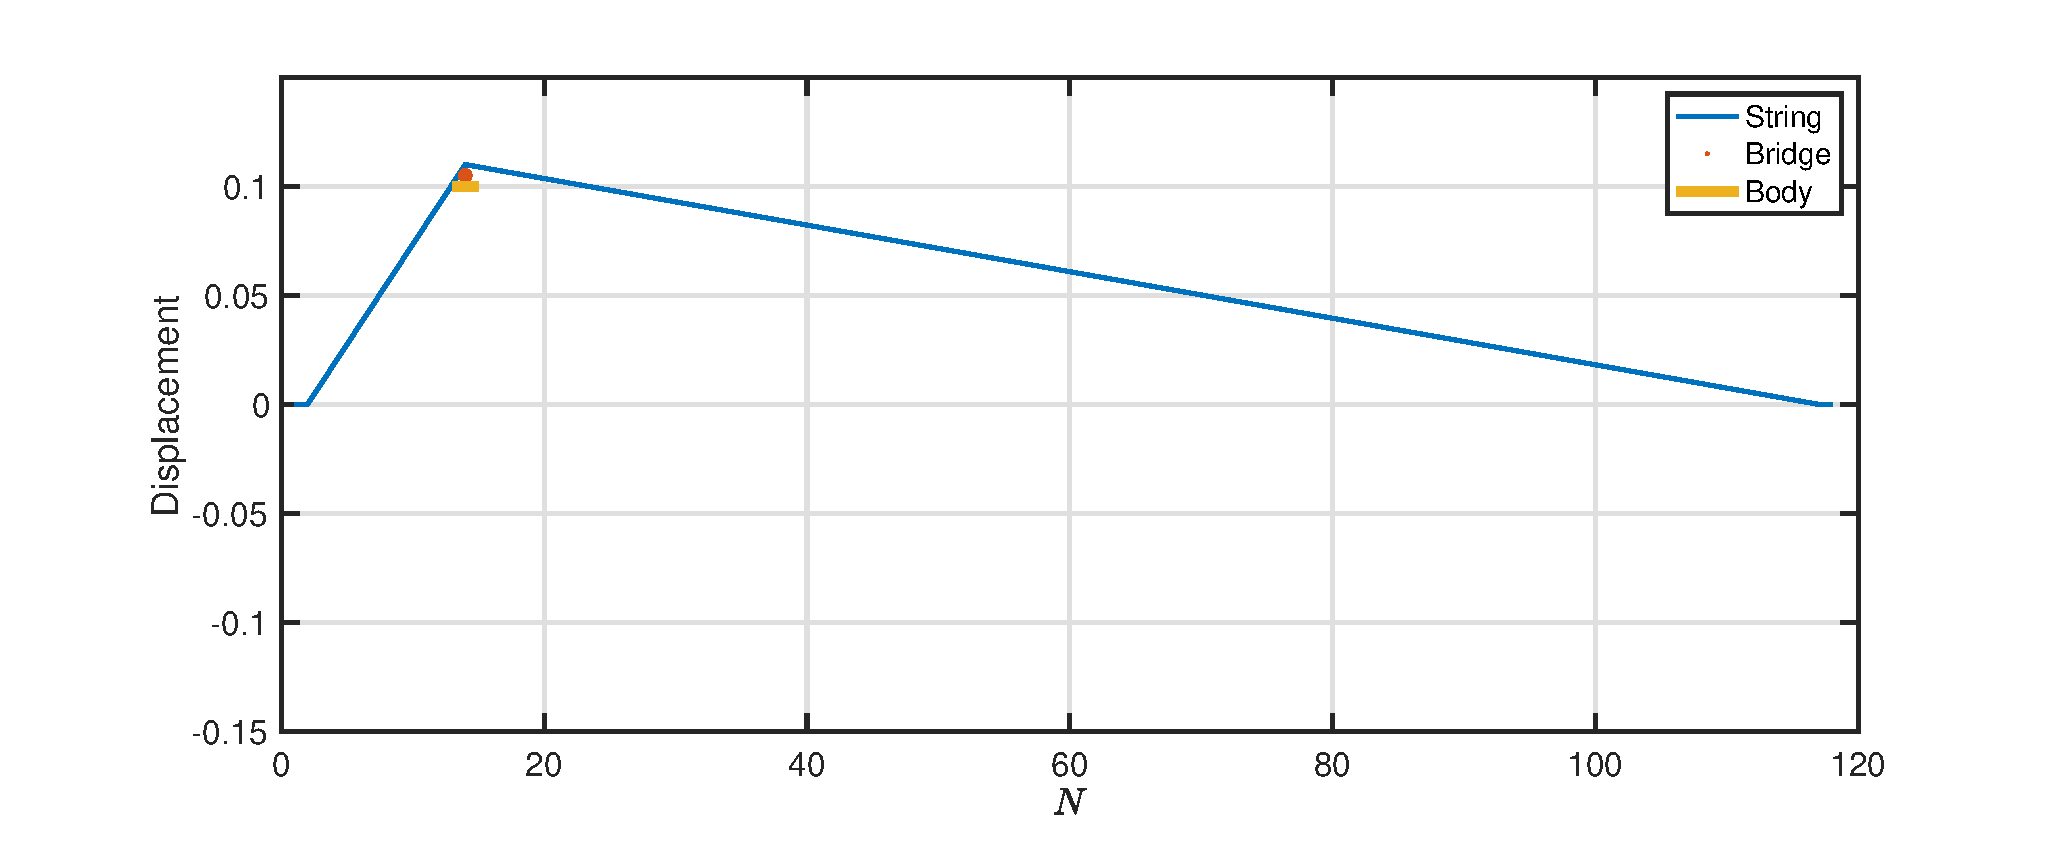
\includegraphics[width=1\columnwidth]{tromba.eps}}
\caption{\label{fig:tromba}{The tromba marina system: a string, a bridge (mass) and body (rigid barrier).}}
\end{figure}

\begin{subnumcases}{\label{eq:trombaSystem}}
    \rho_\text{s} A \delta_{tt}u^n_l & $=T\delta_{xx}u^n_l - EI\delta_{xxxx}u^n_l - J_\text{s}(l_\text{br})F_\alpha$ \\
    M \delta_{tt}w^n &$=-M\omega_0^2w^n + \big(\mu_{t+}\psi^{n-1/2}\big)g^n + F_\alpha$\\
    \rho_\text{p} H \delta_{tt}v^n_{(l,m)} & $ =-D\delta_{\Delta \boxplus}\delta_{\Delta \boxplus}v_{(l,m)}^n - J_\text{p}(l_\text{br},m_\text{br}) \big(\mu_{t+}\psi^{n-1/2}\big)g^n$\\
    \delta_{t+}\psi^{n-1/2} &$= g^n\delta_{t\cdot}\eta_\text{c}^n$\\
    \eta_c^n &$= v_{(l_\text{br},m_\text{br})}^n - w^n$\\
    F_\alpha & $= K_1\mu_{tt}\eta_\text{s}^n + K_3(\eta_\text{s}^n)^2\mu_{t\cdot}\eta_\text{s}^n$\label{eq:fAlpha}\\
    \eta_s^n &$= u_{l_\text{br}}^n - w^n$\label{eq:etaSpring}
\end{subnumcases}
where $D = \frac{EH^3}{12(1-\nu^2)}$. The subscripts $\text{s}$ and $\text{p}$ for $\rho$ denote that it either belongs to the string or the plate. The subscripts $\text{s}$ and $\text{c}$ for $\eta$ denote that it either belongs to the non-linear \underline{s}pring or the \underline{c}ollision.
As done in Section \ref{sec:massString}, the spreading operator $J_\text{s}$ is used to apply the effect of the mass only to grid point $l_\text{br}$ on the string. We now also use the 2D spreading operator $J_\text{p}$ to apply the effect of the mass to grid point $(l_\text{br}, m_\text{br})$

\begin{equation}
J_\text{p}(l_\text{br}, m_\text{br})=
    \begin{cases}
        1/h_\text{p}^2, & l = l_\text{br} \wedge m = m_\text{br}\\
        0, & \text{otherwise}
    \end{cases}
\end{equation}
Expanding the operators of \eqref{eq:fAlpha} and rewriting for $\eta_\text{s}$ yields:
\begin{equation}\label{eq:etaNextSpring}
    \eta_\text{s}^{n+1} = \frac{F_\alpha}{\Phi}-\frac{K_1\eta_\text{s}^n}{2\Phi}-\eta_\text{s}^{n-1},
\end{equation}
where 
\begin{equation}
    \Phi = \frac{K_1}{4}+\frac{K_3(\eta_\text{s}^n)^2}{2}.
\end{equation}
We can define intermediate states (at the bridge) for the connected components, i.e., $u^\text{I}_\text{br}$ and $w^\text{I}$ (where the subscript $\text{br}$ is short for $l_\text{br}$) that exclude the effects of spring and collision forces:
\begin{subequations}\label{eq:intermediate}
    \begin{align}
        u^\text{I}_\text{br} &= 2u_\text{br}^n-u_\text{br}^{n-1}+\frac{Tk^2}{\rho_\text{s}A}\delta_{xx}u_\text{br}^n-\frac{EIk^2}{\rho_\text{s}A}\delta_{xxxx}u_\text{br}^n\\
        w^\text{I} &= 2w^n-w^{n-1}-k^2\omega_0^2w^n%\\
        % v^\text{I}_{\text{br}} &= 2v_{\text{br}}^n-v_{\text{br}}^{n-1}-\frac{Dk^2}{\rho_\text{p}H}\delta_{\Delta\boxplus}\delta_{\Delta\boxplus}v_{\text{br}}^n \label{eq:noDampPlateIntermediate}
    \end{align}
\end{subequations}
Then, looking at the full system in \eqref{eq:trombaSystem} we get that
\begin{subequations}\label{eq:systemNP1NoDamp}
    \begin{align}
        u_\text{br}^{n+1}&=u_\text{br}^\text{I} - \frac{F_\alpha k^2}{h_\text{s}\rho_\text{s}A}\\
        w^{n+1} &= w^\text{I} + \frac{k^2}{M}\big((\mu_{t+}\psi^{n-1/2})g^n + F_\alpha\big)\label{eq:massNP1}\\
        % v_\text{br}^{n+1} &= v_\text{br}^\text{I} - \frac{k^2}{h_\text{p}^2\rho_\text{p}H}\big(\mu_{t+}\psi^{n-1/2}\big)g^n\label{eq:plateNP1}
    \end{align}
\end{subequations}
% (we do not need \eqref{eq:plateNP1} here, but has been written down for clarity). 
As the $(\mu_{t+}\psi^{n-1/2})$-term in \eqref{eq:massNP1} also contains $w^{n+1}$ we need to solve for this
\begin{align}\label{eq:solveForNP1}
    \frac{M}{k^2}w^{n+1} &= \frac{M}{k^2}w^\text{I}+\frac{(g^n)^2}{4}(\eta_\text{c}^{n+1}-\eta_\text{c}^{n-1})+\psi^{n-1/2}g^n+F_\alpha\nonumber\\
    \frac{M}{k^2}w^{n+1} &= \frac{M}{k^2}w^\text{I}+\frac{(g^n)^2}{4}\big((v^{n+1}_\text{br} - w^{n+1}\big)-\eta_\text{c}^{n-1})+\psi^{n-1/2}g^n+F_\alpha\nonumber\\
    \left(\frac{M}{k^2}+\frac{(g^n)^2}{4}\right)w^{n+1} &= \frac{M}{k^2}w^\text{I}+\frac{(g^n)^2}{4}(v^{n+1}_\text{br}-\eta_\text{c}^{n-1})+\psi^{n-1/2}g^n+F_\alpha\nonumber\\
    w^{n+1} &= \frac{\frac{M}{k^2}w^\text{I}+\frac{(g^n)^2}{4}(v^{n+1}_\text{br}-\eta_\text{c}^{n-1})+\psi^{n-1/2}g^n+F_\alpha}{\frac{M}{k^2}+\frac{(g^n)^2}{4}}
\end{align}
Then writing out \eqref{eq:etaSpring} for $\eta_\text{s}^{n+1}$ gives
\begin{equation}\label{eq:etaNextSpringFDS}
    \eta_\text{s}^{n+1} =u^\text{I}_\text{br}-\frac{F_\alpha k^2}{h_\text{s}\rho_\text{s}A}-\frac{\frac{M}{k^2}w^\text{I}+\frac{(g^n)^2}{4}(v_{\text{br}}^{n+1}-\eta_\text{c}^{n-1}) + \psi^{n-1/2}g^n + F_\alpha}{\frac{M}{k^2}+\frac{(g^n)^2}{4}}.
\end{equation}
Setting Equations \eqref{eq:etaNextSpring} and \eqref{eq:etaNextSpringFDS} equal to each other, we can solve for $F_\alpha$
\begin{align}
        \frac{F_\alpha}{\Phi}-\frac{K_1\eta_\text{s}^n}{2\Phi}-\eta_\text{s}^{n-1}&= u^\text{I}_\text{br}-\frac{F_\alpha k^2}{h_\text{s}\rho_\text{s}A}-\frac{\frac{M}{k^2}w^\text{I}+\frac{(g^n)^2}{4}(v_{\text{br}}^{n+1}-\eta_\text{c}^{n-1}) + \psi^{n-1/2}g^n + F_\alpha}{\frac{M}{k^2}+\frac{(g^n)^2}{4}}\nonumber\\
    \Psi F_\alpha &= \frac{K_1\eta_\text{s}^n}{2\Phi}+\eta_\text{c}^{n-1}+ u^\text{I}_\text{br}-\frac{\frac{M}{k^2}w^\text{I}+\frac{(g^n)^2}{4}(v_{\text{br}}^{n+1}-\eta_\text{c}^{n-1}) + \psi^{n-1/2}g^n}{\frac{M}{k^2}+\frac{(g^n)^2}{4}}
\end{align}
where 
\begin{equation}
    \Psi = \frac{1}{\Phi} + \frac{k^2}{h_\text{s}\rho_\text{s}A}+\frac{1}{\frac{M}{k^2}+\frac{(g^n)^2}{4}}.
\end{equation}
If we factor out the effect of unknown $v_\text{br}^{n+1}$ we get
\begin{equation}
\begin{aligned}
    F_\alpha &= F_\alpha'- \Theta v_{\text{br}}^{n+1} \quad \text{where}\\
    F_\alpha' &= \Bigg(\frac{K_1\eta_\text{s}^n}{2\Phi}+\eta_\text{s}^{n-1}+ u^\text{I}_\text{br}
    -\frac{\frac{M}{k^2}w^\text{I}-\frac{(g^n)^2}{4}\eta_\text{c}^{n-1} + \psi^{n-1/2}g^n}{\frac{M}{k^2}+\frac{(g^n)^2}{4}}\Bigg) / \Psi \nonumber \\
    \text{and} \quad \Theta &= \frac{\frac{(g^n)^2}{4}}{\Psi(\frac{M}{k^2}+\frac{(g^n)^2}{4})}
    \end{aligned}
\end{equation}
The complete system can then be solved for the bridge by

\begin{align}
\begin{bmatrix}
        u^{n+1}_{l_\text{br}}\\
        w^{n+1}\\
        v^{n+1}_{(l_\text{br}, m_\text{br})}
    \end{bmatrix}
    = 
    \mathbf{A}^{-1}\mathbf{v}
\end{align}
where
\begin{equation}
\begin{gathered}
\mathbf{A} = 
    \begin{bmatrix}
        \frac{\rho_\text{s} A}{k^2} & 0 & - \frac{\Theta}{h_\text{s}}\\
        0 & \frac{M}{k^2}+\frac{(g^n)^2}{4} &\Theta-\frac{(g^n)^2}{4}\\
        0 & -\frac{(g^n)^2}{4h_\text{p}^2} & \frac{\rho_\text{p}H}{k^2} + \frac{(g^n)^2}{4h_\text{p}^2}
    \end{bmatrix}
    \quad \text{and}\\
    \mathbf{v} = 
    \begin{bmatrix}
        \frac{\rho_\text{s} A}{k^2}(2u^n_\text{br}-u_\text{br}^{n-1})+T\delta_{xx}u_\text{br}^n-EI\delta_{xxxx}u_\text{br}^n - F_\alpha'/h_\text{s}\\
        \frac{M}{k^2}(2w^n-w^{n-1})-M\omega_0^2w^n-\frac{(g^n)^2}{4}\eta_\text{c}^{n-1}+\psi^{n-1/2}g^n + F_\alpha'\\
        \frac{\rho_\text{p}H}{k^2}(2v_\text{br}^n-v_\text{br}^{n-1})-D\delta_{\Delta\boxplus}\delta_{\Delta\boxplus}v_\text{br}^n+\Big(\frac{(g^n)^2}{4}\eta_\text{c}^{n-1}-\psi^{n-1/2}g^n\Big)/h_\text{p}^2
    \end{bmatrix}
    \nonumber
\end{gathered}
\end{equation}

\subsection{Adding damping}
Damping can be added to the string, mass and plate. This results in the following system:
\begin{subnumcases}{}
    \rho_\text{s} A \delta_{tt}u^n_l & $=T\delta_{xx}u^n_l - EI\delta_{xxxx}u^n_l - 2\sigma_{0,\text{s}}\delta_{t\cdot}u_l^n+2\sigma_{1,\text{s}}\delta_{t-}\delta_{xx}u_l^n- J_\text{s}(l_\text{br})F_\alpha$ \\
    M \delta_{tt}w^n &$=-M\omega_0^2w^n - R \delta_{t\cdot}w^n+ \big(\mu_{t+}\psi^{n-1/2}\big)g^n + F_\alpha$\\
    \begin{aligned}
    &\rho_\text{p} H \delta_{tt}v^n_{(l,m)}\\ 
    & 
    \end{aligned}
    & $\begin{aligned} 
    =&-D\delta_{\Delta \boxplus}\delta_{\Delta \boxplus}v_{(l,m)}^n - 2\sigma_{0, \text{p}}\delta_{t\cdot}v^n_{(l,m)} + 2\sigma_{1, \text{p}}\delta_{t-}\delta_{\Delta\boxplus}v_(l,m)^n \\
    &- J_\text{p}(l_\text{br},m_\text{br}) \big(\mu_{t+}\psi^{n-1/2}\big)g^n
    \end{aligned}$\\
    \delta_{t+}\psi^{n-1/2} &$= g^n\delta_{t\cdot}\eta_\text{c}^n$\\
    \eta_\text{c}^n &$= v_{(l_\text{br},m_\text{br})}^n - w^n$\\
    F_\alpha & $= K_1\mu_{tt}\eta_\text{s}^n + K_3(\eta_\text{s}^n)^2\mu_{t\cdot}\eta_\text{s}^n + 2 \sigma_\times\delta_{t\cdot}\eta_\text{s}^n$\label{eq:fAlphaDamp}\\
    \eta_s^n &$= u_{l_\text{br}}^n - w^n$\label{eq:etaSpringDamp}
\end{subnumcases}
where $\sigma_0$ and $\sigma_1$ are frequency independent and frequency dependent damping coefficients and $R$ is a damping coefficient for the bridge (mass). If we, like in \eqref{eq:etaNextSpring}, solve for $\eta_\text{s}^{n+1}$, this gives
\begin{equation}\label{eq:etaSpringNextDamp}
    \eta^{n+1}_\text{s} = \frac{F_\alpha - K_1\eta^n_\text{s} / 2  - \Phi_-\eta_\text{s}^{n-1}}{\Phi_+}
\end{equation}
where
\begin{equation}
    \Phi_+ = \frac{K_1}{4}+\frac{K_3(\eta^n_\text{s})^2}{2} + \frac{\sigma_\times}{k} \quad \text{and} \quad \Phi_- = \frac{K_1}{4}+\frac{K_3(\eta^n_\text{s})^2}{2} - \frac{\sigma_\times}{k}.
\end{equation}
As some of the added terms include the state (of a grid point) at the next sample ($n+1$), we add the terms to and slightly rewrite \eqref{eq:intermediate} to yield

\begin{subequations}\label{eq:intermediateDamp}
    \begin{align}
        u^\text{I}_\text{br}& = \frac{\frac{\rho_\text{s} A}{k^2}(2u_\text{br}^n-u_\text{br}^{n-1})+T\delta_{xx}u_\text{br}^n-EI\delta_{xxxx}u_\text{br}^n + \frac{\sigma_{0,\text{s}}}{k}u_\text{br}^{n-1} + 2\sigma_{1,\text{s}}\delta_{t-}\delta_{xx}u^n_\text{br}}{\frac{\rho_\text{s}A}{k^2} + \frac{\sigma_{0,\text{s}}}{k}} \\
        w^\text{I} & = \frac{\frac{M}{k^2}(2w^n-w^{n-1})-M\omega_0^2w^n+\frac{R}{2k}w^{n-1}}{\frac{M}{k^2} + \frac{R}{2k}}\\
        v^\text{I}_{\text{br}} & = \frac{\frac{\rho_\text{p}H}{k^2}(2v_{\text{br}}^n-v_{\text{br}}^{n-1})-D\delta_{\Delta\boxplus}\delta_{\Delta\boxplus}v_{\text{br}}^n+\frac{\sigma_{0,\text{p}}}{k}v^{n-1}_\text{br}+ 2\sigma_{1,\text{p}}\delta_{t-}\delta_{xx}v^n_\text{br}}{\frac{\rho_\text{p}H}{k^2}+\frac{\sigma_{0,\text{p}}}{k}}
    \end{align}
\end{subequations}
\textbf{$\Leftarrow$ probably don't include the divisions here as that will already happen when doing the matrix division}\\
and similarly to \eqref{eq:systemNP1NoDamp} we can rewrite the individual connected parts of the system at $n+1$ as
\begin{subequations}
\begin{align}
    u_\text{br}^{n+1}&=u_\text{br}^\text{I} - \frac{F_\alpha}{h_\text{s}(\frac{\rho_\text{s}A}{k^2}+\frac{\sigma_{0,\text{s}}}{k})}\\
        w^{n+1} &= w^\text{I} + \frac{(\mu_{t+}\psi^{n-1/2})g^n + F_\alpha}{\frac{M}{k^2}+\frac{R}{2k}}\label{eq:wNP1Damp}%\\
        % v_\text{br}^{n+1} &= v_\text{br}^\text{I} - \frac{\big(\mu_{t+}\psi^{n-1/2}\big)g^n}{h_\text{p}^2(\frac{\rho_\text{p}H}{k^2}+\frac{\sigma_{0,\text{p}}}{k})}
        \end{align}
\end{subequations}
and in a similar fashion as \eqref{eq:solveForNP1}, we solve \eqref{eq:wNP1Damp} for $w^{n+1}$:
\begin{equation}
    w^{n+1} = \frac{\left(\frac{M}{k^2}+\frac{R}{2k}\right)w^\text{I}-\frac{(g^n)^2}{4}\eta_\text{c}^{n-1}+\psi^{n-1/2}g^n+F_\alpha}{\frac{M}{k^2}+\frac{R}{2k}+\frac{(g^n)^2}{4}}
\end{equation}
Setting \eqref{eq:etaSpringDamp} (at $n+1$) and \eqref{eq:etaSpringNextDamp} equal to each other and solving for $F_\alpha$ yields
\begin{align}
    F_\alpha = &F'_\alpha - \Theta v^{n+1}_\text{br} \quad \text{where}\\
    F_\alpha' =& \Bigg(\frac{K_1\eta^n_\text{s}}{2\Phi_+}+\frac{\Phi_-}{\Phi_+}\eta_\text{s}^{n-1}+u^\text{I}_\text{br}-\frac{\Big(\frac{M}{k^2}+\frac{R}{2k}\Big)w^\text{I}-\frac{(g^n)^2}{4}\eta_\text{c}^{n-1}+\psi^{n-1/2}g^n}{\frac{M}{k^2}+\frac{R}{2k}+\frac{(g^n)^2}{4}}\Bigg)/\Psi\\
    \text{and} \quad \quad \Theta &= \frac{\frac{(g^n)^2}{4}}{\Psi(\frac{M}{k^2} + \frac{R}{2k} + \frac{(g^n)^2}{4})}\quad =\quad \frac{(g^n)^2 k^2}{\Psi (4M+2Rk+(g^n)^2k^2)},
\end{align}
where 
\begin{equation}
    \Psi = \frac{1}{\Phi_+} +  \frac{1}{h_\text{s}\Big(\frac{\rho_\text{s}A}{k^2} + \frac{\sigma_0}{k}\Big)}+\frac{1}{\frac{M}{k^2}+\frac{R}{2k} + \frac{(g^n)^2}{4}}.
\end{equation}

The force excluding the effect of unknown $v_\text{br}^{n+1}$, and defining the following unchanging (and thus pre-computable) variables
\begin{align}
    \theta_\text{s} &= h_\text{s}(\rho_\text{s}A+\sigma_{0,\text{s}}k),\\
    \theta_\text{b} &= 4M + 2Rk
\end{align}
$F_\alpha'$, can be rewritten to a formula with only one division:
\begin{align}\label{eq:fAlphaOneDivision}
    F_\alpha' &= \frac{\begin{gathered}(\theta_\text{b} + (g^n)^2k^2)(2kK_1\eta_\text{s}^n+\phi_-\eta_\text{s}^{n-1} +\phi_+u^\text{I}_\text{br})
    - \phi_+\Big(\theta_\text{b}w^\text{I} - (g^n)^2k^2\eta_\text{c}^{n-1} + 4k^2\psi^{n-1/2}g^n\Big)\end{gathered}}{\phi_+\Psi(\theta_\text{b}+ (g^n)^2k^2)}\\
    &=\frac{\left\{
    \begin{gathered}
    \phi_+\theta_\text{s}(\theta_\text{b}+(g^n)^2k^2)\Big[(\theta_\text{b}+(g^n)^2k^2)(2kK_1\eta_\text{s}^n+\phi_-\eta_\text{s}^{n-1}+\phi_+u_\text{br}^\text{I})\\
    -\phi_+\Big(\theta_\text{b}w^\text{I}-(g^n)^2k^2\eta_\text{c}^{n-1}+4k^2\psi^{n-1/2}g^n\Big)\Big]
    \end{gathered}
    \right\}}{
    \begin{gathered}\phi_+(\theta_\text{b}+(g^n)^2k^2)\left(\phi_+k^2\Big(\theta_\text{b}+(g^n)^2k^2 + 4\theta_\text{s}\Big)+
    4k\theta_\text{s}(\theta_\text{b} +(g^n)^2k^2)\right)
    \end{gathered}}
\end{align}
where 
\begin{equation}
    \phi_+ = k (K_1 + 2 K_3 (\eta_\text{s})^2) + 4 \sigma_\times \quad \text{and} \quad \phi_- = k (K_1 + 2 K_3 (\eta_\text{s})^2) - 4 \sigma_\times
\end{equation}
and 
\begin{equation}
    \Theta = \frac{(\phi_+ \theta_\text{s}g^2k^2)}{\phi_+ k^2(\theta_\text{b}+ g^2k^2 + 4\theta_\text{s}) + 4k\theta_\text{s}(\theta_\text{b} + g^2k^2)}
\end{equation}
The complete system can then be solved for the bridge by

\begin{align}
\begin{bmatrix}
        u^{n+1}_\text{br}\\
        w^{n+1}\\
        v^{n+1}_\text{br}
    \end{bmatrix}
    = 
    \mathbf{A}^{-1}\mathbf{v}
\end{align}
where
\begin{equation}
\begin{gathered}
\mathbf{A} = 
    \begin{bmatrix}
        \frac{\rho_\text{s} A}{k^2} + \frac{\sigma_{0,\text{s}}}{k} & 0 & - \frac{\Theta}{h_\text{s}}\\
        0 & \frac{M}{k^2}+\frac{R}{2k}+\frac{(g^n)^2}{4} &\Theta-\frac{(g^n)^2}{4}\\
        0 & -\frac{(g^n)^2}{4h_\text{p}^2} & \frac{\rho_\text{p}H}{k^2} + \frac{\sigma_{0,\text{p}}}{k} + \frac{(g^n)^2}{4h_\text{p}^2}
    \end{bmatrix}
    \quad \text{and}\\
    \mathbf{v} = 
    \begin{bmatrix}
        \frac{\rho_\text{s} A}{k^2}(2u^n_\text{br}-u_\text{br}^{n-1})+T\delta_{xx}u_\text{br}^n-EI\delta_{xxxx}u_\text{br}^n + \frac{\sigma_{0,\text{s}}}{k}u_\text{br}^{n-1} + 2\sigma_{1,\text{s}}\delta_{t-}\delta_{xx}u_\text{br}^n - \frac{F_\alpha'}{h_\text{s}}\\
        \frac{M}{k^2}(2w^n-w^{n-1})-M\omega_0^2w^n + \frac{R}{2k}w^{n-1}-\frac{(g^n)^2}{4}\eta^{n-1}+\psi^{n-1/2}g^n + F_\alpha'\\
        \frac{\rho_\text{p}H}{k^2}(2v_\text{br}^n-v_\text{br}^{n-1})-D\delta_{\Delta\boxplus}\delta_{\Delta\boxplus}v_\text{br}^n+ \frac{\sigma_{0,\text{p}}}{k}v^{n-1}_\text{br} + 2\sigma_{1,\text{p}}\delta_{t-}\delta_{\Delta\boxplus}v^n_\text{br} + \Big(\frac{(g^n)^2}{4}\eta^{n-1}-\psi^{n-1/2}g^n\Big)/h_\text{p}^2
    \end{bmatrix}
    \nonumber
\end{gathered}
\end{equation}
\subsection{Writing for C++}
An essential aspect of real-time sound synthesis is to reduce the number of operations as much as possible. 
\begin{itemize}
    \item Precalculating time-invariant variables
    \item Group changing variables together
\end{itemize}
The following equations are identical to the ones found in \eqref{eq:intermediateDamp} but with the grid variables ($u_l^n$) factored out (rewritten to have the least amount of operations). Using the following short hand notations
\begin{equation}
\lambda^2 \triangleq \frac{Tk^2}{\rho_\text{s}Ah^2}\ , \quad \mu_\text{s}^2 \triangleq \frac{EIk^2}{\rho_\text{s}Ah^4},\ \quad \mu_\text{p}^2 \triangleq \frac{Dk^2}{\rho_\text{s}Hh^4}
\end{equation}
and for the plate grid functions
\begin{equation}
    \begin{aligned}
    v_\text{br}^n &\triangleq v_{l_\text{br},m_\text{br}}^n\\
    v_{\text{br}\pm1}^n &\triangleq (v_{l_\text{br}+1,m_\text{br}}^n+v_{l_\text{br},m_\text{br}+1}^n+v_{l_\text{br}-1,m_\text{br}}^n+v_{l_\text{br},m_\text{br}-1}^n)\\
    v_{\text{br}\pm 2}^n &\triangleq (v_{l_\text{br}+2,m_\text{br}}^n+v_{l_\text{br},m_\text{br}+2}^n+v_{l_\text{br}-2,m_\text{br}}^n+v_{l_\text{br},m_\text{br}-2}^n)\\
    v_{l_\text{br}\pm1, m_\text{br}\pm1}^n &\triangleq (v_{l_\text{br}+1,m_\text{br}+1}^n+v_{l_\text{br}+1,m_\text{br}-1}^n+v_{l_\text{br}-1,m_\text{br}+1}^n+v_{l_\text{br}-1,m_\text{br}-1}^n)
    \end{aligned}
\end{equation}
and using $\sigma_{0,\text{s}} = \sigma_{0,\text{s}} / \rho_\text{s}A$, $\sigma_{1,\text{s}} = \sigma_{1,\text{s}} / \rho_\text{s}A$, $\sigma_{0,\text{p}}  = \sigma_{0,\text{p}} / \rho_\text{p}H$ and $\sigma_{2,\text{p}}  = \sigma_{2,\text{p}} / \rho_\text{p}H$ we get
\begin{subequations}\label{eq:intermediateDampFact}
    \begin{align}
        u^\text{I}_\text{br} = &\Big[(2-2\lambda^2-\mu_\text{s}^2-\frac{4\sigma_{1,\text{s}}k}{h^2})u_l^n + (\lambda^2 + 4\mu_\text{s}^2+\frac{2\sigma_{1,\text{s}}k}{h^2})(u_{\text{br}+1}^n + u_{\text{br}-1}^n)\nonumber\\
        &+ (-\mu_\text{s}^2)(u_{\text{br}+2}^n+u_{\text{br}-2}^n)+ (-1 + \sigma_{0,\text{s}}k+\frac{4\sigma_{1,\text{s}}k}{h^2})u_l^{n-1}+(-\frac{2\sigma_{1,\text{s}}k}{h^2})(u_{\text{br}+1}^{n-1} + u_{\text{br}-1}^{n-1})\Big]\\
        &/ \Big[1 + \sigma_{0,\text{s}}k\Big] \nonumber\\
        w^\text{I} = & \frac{(2-\omega_0^2k^2)w^n+(-1+\frac{Rk}{2M})w^{n-1}}{1+\frac{Rk}{2M}}\\
        v^\text{I}_\text{br} =& \Big[(2-20\mu^2_\text{p}-\frac{8\sigma_{1,\text{p}}k}{h^2})v_\text{br}^n+(8\mu_\text{p}^2+\frac{2\sigma_{1,\text{p}}k}{h^2})v_{\text{br}\pm1}^n+ (-2\mu_\text{p}^2)v_{l_\text{br}\pm1,m_\text{br}\pm1}^n+(-\mu_\text{p}^2)v_{\text{br}\pm2}^n\\
        &+(-1 + \frac{8\sigma_{1,\text{p}}k}{h^2})v_\text{br}^{n-1}+(-\frac{2\sigma_{1,\text{p}}k}{h^2})v_{\text{br}\pm1}^{n-1}\Big]/\Big[1+\sigma_{0,\text{p}}k\Big]\nonumber
    \end{align}
\end{subequations}
Again, as done in \eqref{eq:systemNP1NoDamp} the individual components at $n+1$ are \textbf{I DO INCUDE THE PLATE HERE}
\begin{subequations}
\begin{align}
    u_\text{br}^{n+1}&=u_\text{br}^\text{I} - \frac{F_\alpha k^2}{h_\text{s}\rho_\text{s}A(1+\sigma_{0,\text{s}}k)}\\
        w^{n+1} &= w^\text{I} + \frac{((\mu_{t+}\psi^{n-1/2})g^n + F_\alpha)k^2}{M (1+\frac{Rk}{2M})}\\
        v_\text{br}^{n+1} &= v_\text{br}^\text{I} - \frac{\big(\mu_{t+}\psi^{n-1/2}\big)g^nk^2}{h_\text{p}^2\rho_\text{p}H(1+\sigma_{0,\text{p}}k)}
        \end{align}
\end{subequations}
and as in \eqref{eq:solveForNP1} we solve for $w^{n+1}$
\begin{equation}
    w^{n+1} = \frac{M(1+\frac{Rk}{2M})w^\text{I}+k^2\left(\frac{(g^n)^2}{4}(v_\text{br}^{n+1}-\eta_\text{c}^{n-1})+\psi^{n-1/2}g^n+F_\alpha\right)}{M(1+\frac{Rk}{2M})+\frac{(g^n)^2k^2}{4}}.
\end{equation}
We can use this to solve for $F_\alpha$ which can be shown to be identical to \eqref{eq:fAlphaOneDivision}.

Then, the complete rewritten system can then be solved for the bridge by

\begin{align}
\begin{bmatrix}
        u^{n+1}_{l_\text{br}}\\
        w^{n+1}\\
        v^{n+1}_{(l_\text{br}, m_\text{br})}
    \end{bmatrix}
    = 
    \mathbf{A}^{-1}\mathbf{v}
\end{align}
where
\begin{equation}
\begin{gathered}
\mathbf{A} = 
    \begin{bmatrix}
        1+\sigma_{0,\text{s}}k & 0 & - \frac{\Theta}{\rho_\text{s}Ah_\text{s}}\\
        0 & M(1+\frac{Rk}{2M}) + \frac{(g^n)^2k^2}{4} &\Theta-\frac{(g^n)^2k^2}{4}\\
        0 & -\frac{(g^n)^2k^2}{4h_\text{p}^2} & \rho_\text{p}H(1+\sigma_{0,\text{p}}k) + \frac{(g^n)^2k^2}{4h_\text{p}^2}
    \end{bmatrix}
    \quad \text{and}\\
    \mathbf{v} = 
    \begin{bmatrix}
        (1+\sigma_{0,\text{s}}k)u_\text{br}^\text{I} - \frac{F_\alpha'k^2}{h_\text{s}\rho_\text{s}A}\\
        M(1+\frac{Rk}{2M})w^\text{I}+k^2\left(-\frac{(g^n)^2}{4}\eta^{n-1}+\psi^{n-1/2}g^n + F_\alpha'\right)\\
        \rho_\text{p}H(1+\sigma_{0,\text{p}}k)v_\text{br}^\text{I}+\frac{k^2}{h_\text{p}^2}\left(\frac{(g^n)^2}{4}\eta^{n-1}-\psi^{n-1/2}g^n\right)
    \end{bmatrix}
    \nonumber
\end{gathered}
\end{equation}

\subsection{Energy Analysis}
\section{Tromba Marina: Collision rather than connection}
If we assume the string and the bridge to be ``connected" using an alternative form of \eqref{eq:potential} (as per Eq. (14) in \cite{Bilbao2019}) we obtain
\begin{equation}\label{eq:potentialConnection}
    \phi'(\eta) = K[|\eta| - \epsilon]_+^\alpha\text{sgn}(\eta) \xrightarrow{\ \ \epsilon = 0\ \ } K|\eta|^\alpha\text{sgn}(\eta).
\end{equation}
Taking the absolute value of $\eta$ means that there will always be a force which is directed by a multiplication with the sign of $\eta$. Knowing that $\text{sgn}(x) = x/|x|$ we can rewrite \eqref{eq:potentialConnection} to
\begin{equation}
    \phi'(\eta)=K|\eta|^\alpha\frac{\eta}{|\eta|},
\end{equation}
which, after taking the antiderivative becomes (see Appendix \ref{app:integration} for the steps)
\begin{equation}
    \phi(\eta)= \frac{K}{\alpha+1}|\eta|^{\alpha+1}.
\end{equation}
Like in \eqref{eq:gn}, $g^n$ can be defined as:
\begin{equation}
    g^n = \frac{K|\eta^n|^\alpha \text{sgn}(\eta^n)}{\sqrt{\frac{2K|\eta^n|^{\alpha+1}}{\alpha+1}}}\quad= \text{sgn}(\eta^n)\sqrt{\frac{K(\alpha+1)}{2}}|\eta^n|^{\frac{\alpha-1}{2}}\quad= \eta^n\sqrt{\frac{K(\alpha+1)}{2}}|\eta^n|^{\frac{\alpha-3}{2}}
\end{equation}
This definition will be used for the connection between the string and the bridge, further defined as $g_1$ and the collision between the bridge and the body will be defined as $g_2$. The complete system will then be:

\textit{ Note: from here I'll be writing in the style which will be used for the journal paper. This includes multiplying the string and plate damping terms with their respective $\rho$'s and $A$ or $H$, and using (complete system) partial differential operators}
$\mathscr{abcdefg}$
\begin{subnumcases}{}
     \ell_\text{s}u_l^n & $= J_\text{s}(l_\text{br}) \big(\mu_{t+}\psi_1^{n-1/2}\big)g_1^n$ \\
    \ell_\text{b}w^n & $= - \big(\mu_{t+}\psi_1^{n-1/2}\big)g_1^n+ \big(\mu_{t+}\psi_2^{n-1/2}\big)g_2^n$\\
    \ell_\text{p} v^n_{(l,m)} & $ = - J_\text{p}(l_\text{br},m_\text{br}) \big(\mu_{t+}\psi_2^{n-1/2}\big)g_2^n$\\
    \delta_{t+}\psi_1^{n-1/2} &$= g_1^n\delta_{t\cdot}\eta_1^n$\\
    \delta_{t+}\psi_2^{n-1/2} &$= g_2^n\delta_{t\cdot}\eta_2^n$\\
    \eta_1^n &$= w^n - u_\text{br}^n$\label{eq:eta1Col}\\
    \eta_2^n &$= v_\text{br}^n - w^n$\label{eq:eta2Col}
\end{subnumcases}
where
\begin{subequations}\label{eq:fdsOperators}
\begin{align}
\ell_\text{s} &=\rho_\text{s}A\delta_{tt}- T\delta_{xx} + EI\delta_{xxxx}+ 2\rho_\text{s}A\sigma_{0,\text{s}}\delta_{t\cdot}-2\rho_\text{s}A\sigma_{1,\text{s}}\delta_{t-}\delta_{xx}\\
    \ell_\text{b} &= M\delta_{tt} + M\omega_0^2 + MR \delta_{t\cdot}\\
    \ell_\text{p} &= \rho_\text{p} H \delta_{tt} + D\delta_{\Delta \boxplus}\delta_{\Delta \boxplus} + 2\rho_\text{p}H\sigma_{0, \text{p}}\delta_{t\cdot} - 2\rho_\text{p}H\sigma_{1, \text{p}}\delta_{t-}\delta_{\Delta\boxplus}
    \end{align}
\end{subequations}
    

The complete system can then be solved for the bridge by

\begin{align}
\begin{bmatrix}
        u^{n+1}_\text{br}\\
        w^{n+1}\\
        v^{n+1}_\text{br}
    \end{bmatrix}
    = 
    \mathbf{A}^{-1}\mathbf{v}
\end{align}
where
\begin{equation}
\begin{gathered}
\mathbf{A} = 
    \begin{bmatrix}
        \frac{\rho_\text{s} A}{k^2} + \frac{\rho_\text{s}A\sigma_{0,\text{s}}}{k} + \frac{(g_1^n)^2}{4h_\text{s}} & -\frac{(g_1^n)^2}{4h_\text{s}} & 0 \\
        -\frac{(g_1^n)^2}{4} & \frac{M}{k^2}+\frac{MR}{2k}+\frac{(g_1^n)^2}{4}+\frac{(g_2^n)^2}{4} &-\frac{(g_2^n)^2}{4}\\
        0 & -\frac{(g_2^n)^2}{4h_\text{p}^2} & \frac{\rho_\text{p}H}{k^2} + \frac{\rho_\text{p}H\sigma_{0,\text{p}}}{k} + \frac{(g^n)^2}{4h_\text{p}^2}
    \end{bmatrix}
    \quad \text{and}\\
    \mathbf{v} = 
    \begin{bmatrix}
        \frac{\rho_\text{s} A}{k^2}(2u^n_\text{br}-u_\text{br}^{n-1})+T\delta_{xx}u_\text{br}^n-EI\delta_{xxxx}u_\text{br}^n + \frac{\rho_\text{s} A\sigma_{0,\text{s}}}{k}u_\text{br}^{n-1} + 2\rho_\text{s} A\sigma_{1,\text{s}}\delta_{t-}\delta_{xx}u_\text{br}^n -\left(\frac{(g_1^n)^2}{4}\eta_1^{n-1}-\psi_1^{n-1/2}g_1^n\right)/h_\text{s}\\
        \frac{M}{k^2}(2w^n-w^{n-1})-M\omega_0^2w^n + \frac{MR}{2k}w^{n-1}+\frac{(g_1^n)^2}{4}\eta_1^{n-1}-\psi_1^{n-1}g_1^n-\frac{(g_2^n)^2}{4}\eta_2^{n-1}+\psi_2^{n-1/2}g_2^n\\
        \frac{\rho_\text{p}H}{k^2}(2v_\text{br}^n-v_\text{br}^{n-1})-D\delta_{\Delta\boxplus}\delta_{\Delta\boxplus}v_\text{br}^n+ \frac{\rho_\text{p}H\sigma_{0,\text{p}}}{k}v^{n-1}_\text{br} + 2\rho_\text{p} H\sigma_{1,\text{p}}\delta_{t-}\delta_{\Delta\boxplus}v^n_\text{br} + \Big(\frac{(g^n)^2}{4}\eta^{n-1}-\psi^{n-1/2}g^n\Big)/h_\text{p}^2
    \end{bmatrix}
    \nonumber
\end{gathered}
\end{equation}
It is also possible to solve for  $\delta_{t\cdot}\eta_1^n$ and $\delta_{t\cdot}\eta_2^n$ instead. Recalling \eqref{eq:eta1Col} and \eqref{eq:eta2Col}, we know that the following has to be true:

\begin{equation}
\begin{aligned}
    \delta_{t\cdot}\eta_1^n &= \delta_{t\cdot}(w^n - u_\text{br}^n) \quad \text{and}\\
    \delta_{t\cdot}\eta_2^n &= \delta_{t\cdot}(v_\text{br}^n - w^n)
    \end{aligned}
\end{equation}
which when (semi)expanded yields:
\begin{equation}\label{eq:expandedEtas}
\begin{aligned}
    2k\delta_{t\cdot}\eta_1^n &= w^{n+1}-w^{n-1}-u_\text{br}^{n+1}+u_\text{br}^{n-1} \quad \text{and}\\  2k\delta_{t\cdot}\eta_2^n &= v_\text{br}^{n+1}-v_\text{br}^{n-1}-w^{n+1}+w^{n-1}
    \end{aligned}
\end{equation}
Solving the equations described in \eqref{eq:fdsOperators} for their states at $n+1$ we get:
\begin{subequations}
\begin{align}
    % \left(\frac{\rho_\text{s}A}{k^2}+\frac{\rho_\text{s}A\sigma_{0,\text{s}}}{k}\right) u_\text{br}^{n+1} =
    % &\ \frac{\rho_\text{s}A}{k^2}(2u_\text{br}^n-u_\text{br}^{n-1}) + T\delta_{xx}u_\text{br}^n-EI\delta_{xxxx}u_\text{br}^n+\frac{\rho_\text{s}A\sigma_{0,\text{s}}}{k}u_\text{br}^{n-1}-2\rho_\text{s}A\sigma_{1,\text{s}}\delta_{t-}\delta_{xx}u_\text{br}^n\\
    % & +\frac{1}{h_\text{s}}\left(\frac{(g_1^n)^2k}{2}\delta_{t\cdot}\eta_1^n+\psi_1^{n-1/2}\right)\nonumber\\
    u_\text{br}^{n+1} &= u_\text{br}^\text{I}
     +\frac{k^2}{h_\text{s}\rho_\text{s}A(1+\sigma_{0,\text{s}}k)}\left(\frac{(g_1^n)^2k}{2}\delta_{t\cdot}\eta_1^n+\psi_1^{n-1/2}g_1^n\right)\nonumber\\
    % \left(\frac{M}{k^2}+\frac{MR}{2k}\right)w^{n+1} = &\ \frac{M}{k^2}(2w^n-w^{n-1}) - M\omega_0^2w^n + \frac{MR}{2k}w^{n-1}-\left(\frac{(g_1^n)^2k}{2}\delta_{t\cdot}\eta_1^n+\psi_1^{n-1/2}\right)\\
    % &+\left(\frac{(g_2^n)^2k}{2}\delta_{t\cdot}\eta_2^n+\psi_2^{n-1/2}\right)\nonumber
    w^{n+1} &= w^\text{I}-\frac{k^2}{M\left(1+\frac{Rk}{2}\right)}\left(\frac{(g_1^n)^2k}{2}\delta_{t\cdot}\eta_1^n+\psi_1^{n-1/2}g_1^n\right)+\frac{k^2}{M\left(1+\frac{Rk}{2}\right)}\left(\frac{(g_2^n)^2k}{2}\delta_{t\cdot}\eta_2^n+\psi_2^{n-1/2}g_2^n\right)\nonumber\\
    v_\text{br}^{n+1} &= v_\text{br}^\text{I}-\frac{k^2}{h_\text{p}^2\rho_\text{p}H(1+\sigma_{0,\text{p}}k)}\left(\frac{(g_2^n)^2k}{2}\delta_{t\cdot}\eta_2^n+\psi_2^{n-1/2}g_2^n\right)\nonumber
\end{align}
\end{subequations}
where
\begin{subequations}\label{eq:intermediateColCol}
    \begin{align}
        u^\text{I}_\text{br}& = \frac{2u_\text{br}^n-u_\text{br}^{n-1}+\frac{Tk^2}{\rho_\text{s}A}\delta_{xx}u_\text{br}^n-\frac{EIk^2}{\rho_\text{s}A}\delta_{xxxx}u_\text{br}^n + \sigma_{0,\text{s}}ku_\text{br}^{n-1} + 2\sigma_{1,\text{s}}k^2\delta_{t-}\delta_{xx}u^n_\text{br}}{1 + \sigma_{0,\text{s}}k} \\
        w^\text{I} & = \frac{2w^n-w^{n-1}-k^2\omega_0^2w^n+\frac{Rk}{2}w^{n-1}}{1 + \frac{Rk}{2}}\\
        v^\text{I}_{\text{br}} & = \frac{2v_{\text{br}}^n-v_{\text{br}}^{n-1}-\frac{Dk^2}{\rho_\text{p}H}\delta_{\Delta\boxplus}\delta_{\Delta\boxplus}v_{\text{br}}^n+\sigma_{0,\text{p}}kv^{n-1}_\text{br}+ 2\sigma_{1,\text{p}}k^2\delta_{t-}\delta_{xx}v^n_\text{br}}{1+\sigma_{0,\text{p}}k}
    \end{align}
\end{subequations}
These can then be inserted into \eqref{eq:expandedEtas} and solved for $\delta_{t\cdot}\eta_1^n$ and $\delta_{t\cdot}\eta_2^n$
\begin{equation}
    \begin{bmatrix}
        \delta_{t\cdot}\eta_1^n\\
        \delta_{t\cdot}\eta_2^n
    \end{bmatrix}
    = 
    \mathbf{A}^{-1}\mathbf{v}
\end{equation}
where
\begin{equation}
\begin{gathered}
\mathbf{A} = 
    \begin{bmatrix}
        1 + \frac{(g_1^n)^2k^2}{2M(2+Rk)} + \frac{(g_1^n)^2k^2}{4\rho_\text{s}Ah_\text{s}(1+\sigma_{0,\text{s}}k)} & -\frac{(g_2^n)^2k^2}{2M(2+Rk)} \\
        -\frac{(g_1^n)^2k^2}{2M(2+Rk)} & 1+\frac{(g_2^n)^2k^2}{2M(2+Rk)}+\frac{(g_2^n)^2k^2}{4h_\text{p}^2\rho_\text{p}H(1+\sigma_{0,\text{p}}k)}
    \end{bmatrix}
    \quad \text{and}\\
    \mathbf{v} = 
    \begin{bmatrix}
        \frac{w^\text{I}-w^{n-1}-u_\text{br}^\text{I}+u_\text{br}^{n-1}}{2k} - \frac{k(\psi_1^{n-1/2}g_1^n-\psi_2^{n-1/2}g_2^n)}{M(2+Rk)}-\frac{\psi_1^{n-1/2}g_1^nk}{2\rho_\text{s}Ah_\text{s}(1+\sigma_{0,\text{s}}k)}\\
        \frac{v_\text{br}^\text{I}-v_\text{br}^{n-1}-w^\text{I}+w^{n-1}}{2k}+\frac{k(\psi_1^{n-1/2}g_1^n-\psi_2^{n-1/2}g_2^n)}{M(2+Rk)}-\frac{\psi_2^{n-1/2}g_2^nk}{2h_\text{p}^2\rho_\text{p}H(1+\sigma_{0,\text{p}}k)}
    \end{bmatrix}
    \nonumber
\end{gathered}
\end{equation}
\section{Conclusion}
Using the tools described in this chapter, you can build any system of elements (strings, masses, barriers) and let them collide.
\subsection{Implementation}
Equation \eqref{eq:etaPlus} can be implemented using Matlab's \texttt{subplus} function.

\bibliographystyle{plain}
\bibliography{references}
\appendix
\section{Proof that $\psi\psi' = \phi'$}\label{app:phiPsiProof}
In this appendix, I will prove an equality that Ducceschi presents in \cite{Ducceschi2019} which is crucial to his method:
\begin{equation}\label{eq:equality}
    \psi\psi' = \phi' \Rightarrow \psi\frac{\dot{\psi}}{\dot{\eta}} = \frac{\dot{\phi}}{\dot\eta}\quad \text{where}\quad \psi = \sqrt{2\phi}.
\end{equation}
In discrete time, \eqref{eq:equality} becomes
\begin{equation}\label{eq:discEquality}
    \big(\mu_{t+}\psi^{n-1/2}\big)\,\frac{\delta_{t+}\psi^{n-1/2}}{\delta_{t\cdot}\eta^n} = \frac{\delta_{t+}\phi^{n-1/2}}{\delta_{t\cdot}\eta^n}. 
\end{equation}
Multiplying both sides by $\delta_{t\cdot} \eta^n$ and continuing with the left hand side of \eqref{eq:discEquality}, we can expand its operators:
\begin{equation}
    \begin{aligned}\nonumber
        &\frac{1}{2}\big(\psi^{n+1/2}+\psi^{n-1/2}\big)\frac{1}{k}\big(\psi^{n+1/2}-\psi^{n-1/2}\big) \\
        =\ &\frac{1}{2k}\Big((\psi^{n+1/2})^2 - (\psi^{n-1/2})^2\Big)\\
        =\ &\frac{1}{2k}\bigg(\Big(\sqrt{2\phi^{n+1/2}}\Big)^2 - \Big(\sqrt{2\phi^{n-1/2}}\Big)^2\bigg)\\
        =\ &\frac{1}{k}\Big(\phi^{n+1/2} - \phi^{n-1/2}\Big)\\
        =\ &\delta_{t+}\phi^{n-1/2}
    \end{aligned}
\end{equation}
which, when divided by $\delta_{t\cdot}\eta^n$ again satisfies \eqref{eq:discEquality}.
Knowing that $\sqrt{2\phi}=\psi$
\begin{equation}
    \begin{aligned}
        \psi\psi' &= \phi'\\
        \sqrt{2\phi}\frac{d}{dt}\left[(2\phi\right)^{1/2}] &= \phi'\\
        \sqrt{2\phi}\left(\sqrt{2}\frac{\phi'}{2\sqrt{\phi}}\right) &= \phi'\\
        \sqrt{2\phi}\frac{\phi'}{\sqrt{2\phi}} &= \phi'\\
        \phi' &= \phi'
    \end{aligned}
\end{equation}
\section{Proof that $\delta_{t+}\psi^{n-1/2} = \delta_{t\cdot}\psi^n$}\label{app:operatorProof}
As per Eq. (20) in \cite{Ducceschi2019}, $\psi^{n-1/2} \triangleq \mu_{t-}\psi(\eta^n)$ so,
\begin{equation}
        \delta_{t+}\psi^{n-1/2}=\delta_{t+}(\mu_{t-}\psi(\eta^n))
\end{equation}
Expanding the right-hand side according to \cite{Bilbao2009} Eq. (2.3b), this results in
\begin{equation}
    \begin{aligned}
        \delta_{t+}\psi^{n-1/2}&=\frac{1}{2} \Big(\psi(\eta^n)+\psi(\eta^{n-1})\Big) \\
        &= \frac{1}{k}\left(\frac{1}{2}\Big(\psi(\eta^{n+1})-\psi(\eta^n)+\psi(\eta^n)-\psi(\eta^{n-1})\Big)\right)\\
        &=\frac{1}{2k}\Big(\psi(\eta^{n+1})-\psi(\eta^{n-1})\Big)\\
        &= \delta_{t\cdot}\psi(\eta^n) = \delta_{t\cdot}\psi^n
    \end{aligned}
\end{equation}
\section{Colliding Mass-springs deriviation}\label{app:massMassDeriv}
\begin{align}
    \frac{M_1}{k^2}u^{n+1} &= \frac{M_1}{k^2}(2u^n-u^{n-1})-M_1\omega_1u^n+\Big(\frac{g^n}{4}(\eta^{n+1}-\eta^{n-1})+\psi^{n-1/2}\Big)g^n\nonumber\\
    \frac{M_1}{k^2}u^{n+1} &= \frac{M_1}{k^2}(2u^n-u^{n-1})-M_1\omega_1u^n+\frac{(g^n)^2}{4}(w^{n+1}-u^{n+1}-\eta^{n-1})+\psi^{n-1/2}g^n\nonumber\\
    \bigg(\frac{M_1}{k^2}+\frac{(g^n)^2}{4}\bigg)u^{n+1} &- \frac{(g^n)^2}{4}w^{n+1} = \frac{M_1}{k^2}(2u^n-u^{n-1})-M_1\omega_1u^n-\frac{(g^n)^2}{4}\eta^{n-1}+\psi^{n-1/2}g^n
\end{align}

\begin{align}
    \frac{M_2}{k^2}w^{n+1} &= \frac{M_2}{k^2}(2w^n-w^{n-1})-M_2\omega_2w^n-\Big(\frac{g^n}{4}(\eta^{n+1}-\eta^{n-1})+\psi^{n-1/2}\Big)g^n\nonumber\\
    \frac{M_2}{k^2}w^{n+1} &= \frac{M_2}{k^2}(2w^n-w^{n-1})-M_2\omega_2w^n-\frac{(g^n)^2}{4}(w^{n+1}-u^{n+1}-\eta^{n-1})-\psi^{n-1/2}g^n\nonumber\\
    - \frac{(g^n)^2}{4}u^{n+1} &+ \bigg(\frac{M_2}{k^2}+\frac{(g^n)^2}{4}\bigg)w^{n+1} = \frac{M_2}{k^2}(2w^n-w^{n-1})-M_2\omega_2w^n+\frac{(g^n)^2}{4}\eta^{n-1}-\psi^{n-1/2}g^n
\end{align}

Weird collision case:
\begin{subnumcases}{\label{eq:trombaSystem}}
    \rho A \delta_{tt}u^n_l & $=T\delta_{xx}u^n_l - EI\delta_{xxxx}u^n_l - 2\sigma_0\delta_{t\cdot}u^n_l + 2\sigma_1\delta_{t-}\delta_{xx}u_l^n$ \\
    & $+ J_\text{s}(l_\text{m})(\mu_{t+}\psi_\text{ms}^{n-1/2})g_\text{ms}^n$ \\
    M \delta_{tt}w^n &$=- M \omega_0^2w^n - \big(\mu_{t+}\psi_\text{ms}^{n-1/2}\big)g_\text{ms}^n + \big(\mu_{t+}\psi_\text{mb}^{n-1/2}\big)g_\text{mb}^n$\\
 \delta_{t+}\psi_\text{ms}^{n-1/2} &$= g_\text{ms}^n\delta_{t\cdot}\eta_\text{ms}^n$\\
 \delta_{t+}\psi_\text{mb}^{n-1/2} &$= g_\text{mb}^n\delta_{t\cdot}\eta_\text{mb}^n$\\
    \eta_\text{ms}^n &$= w^n - u_\text{m}^n$\\
    \eta_\text{mb}^n &$= b - w^n$\label{eq:etaSpring}
\end{subnumcases}

\section{Integration by u-substitution}\label{app:integration}
Test
\begin{equation}
\begin{aligned}
    \phi(\eta) &= \int K\frac{\eta}{|\eta|}|\eta|^\alpha d\eta\\
    % \text{u-substitution:}
    &\boxed{
    \begin{aligned}
    u &= |\eta| \\
    \frac{du}{d\eta} &= \frac{\eta}{|\eta|}\\
    d\eta &= \frac{|\eta|}{\eta}du
    \end{aligned}
    }\\
    \end{aligned}\nonumber
\end{equation}
    \begin{equation}
    = K\int \frac{\eta}{|\eta|}u^\alpha\frac{|\eta|}{\eta}du \quad = K\int u^\alpha du \quad = \frac{K}{\alpha + 1}u^{\alpha+1} \quad = \frac{K}{\alpha+1}|\eta|^{\alpha+1}
\end{equation}
\section{Stefans code}
Consider the following system:

\begin{subnumcases}{\label{eq:trombaSystem}}
    M \delta_{tt}w^n &$=- \big(\mu_{t+}\psi_\text{M}^{n-1/2}\big)g_\text{M}^n + \big(\mu_{t+}\psi_\text{B}^{n-1/2}\big)g_\text{B}^n$\label{eq:massStefan}\\
    \rho A \delta_{tt}u^n_l & $=T\delta_{xx}u^n_l+ J_\text{s}(l_\text{br})(\mu_{t+}\psi_\text{M}^{n-1/2})g_\text{M}^n$ \label{eq:stringStefan}\\
 \delta_{t+}\psi_\text{M}^{n-1/2} &$= g_\text{M}^n\delta_{t\cdot}\eta_\text{M}^n$\\
 \delta_{t+}\psi_\text{B}^{n-1/2} &$= g_\text{B}^n\delta_{t\cdot}\eta_\text{B}^n$\\
    \eta_\text{M}^n &$= w^n - u_\text{br}^n$\\
    \eta_\text{B}^n &$= b - w^n$
\end{subnumcases}
%
Because the location of the barrier $b$ is stationary, we know that (also as per \eqref{eq:derEtaEqDerU})
\begin{equation}\label{eq:deltaEtaB}
    \delta_{t\cdot}\eta_\text{B}^n= \delta_{t\cdot}(b-w^n) = \delta_{t\cdot}(-w^n) = -\delta_{t\cdot}w^n.
\end{equation}
Expanding and solving this for $w^{n+1}$ yields
\begin{equation}\label{eq:explicitWNP1}
    w^{n+1} = w^{n-1}-2k\delta_{t\cdot}\eta_B.
\end{equation}
After expansion of \eqref{eq:massStefan}, this can be filled into the equation
\begin{equation}
    \frac{M}{k^2}(w^{n-1}-2k\delta_{t\cdot}\eta_\text{B}-2w^n+w^{n-1})= -\left(\frac{g_\text{M}k}{2}\delta_{t\cdot}\eta_\text{M}^n+\psi_\text{M}^{n-1/2}\right)g_\text{M}^n + \left(\frac{g_\text{B}k}{2}\delta_{t\cdot}\eta_\text{B}^n+\psi_\text{B}^{n-1/2}\right)g_\text{B}^n,
\end{equation}
and can be rewritten to
\begin{equation}
\begin{aligned}
    \frac{2M}{k^2}(w^{n-1}-k\delta_{t\cdot}\eta_\text{B}-w^n)&=\dots\\
    -k\delta_{t\cdot}\eta_\text{B} &= w^n - w^{n-1} + \frac{k^2}{2M}(\dots)\\
    \delta_{t\cdot}\eta_\text{B}&= -\frac{w^n-w^{n-1}}{k}-\frac{k}{2M}(\dots)
        \end{aligned}
\end{equation}
Getting all $\delta_{t\cdot}\eta^n$ terms to the left hand side yields
\begin{equation}\label{eq:solutionMassStefan}
    \left(1+\frac{k^2(g_\text{B}^n)^2}{4M}\right)\delta_{t\cdot}\eta_\text{B}^n-\frac{k^2(g_\text{M}^n)^2}{4M}\delta_{t\cdot}\eta_\text{M}^n = -\frac{w^n-w^{n-1}}{k}+\frac{kg_\text{M}^n\psi^{n-1/2}_M}{2M}-\frac{kg_\text{B}^n\psi_\text{B}^{n-1/2}}{2M}
\end{equation}
The same can be done for \eqref{eq:stringStefan}. Following the same lines as in \eqref{eq:deltaEtaB} we obtain
\begin{equation}
    \delta_{t\cdot}\eta_M^n = \delta_{t\cdot}(w^n-u_\text{br}^n)=\frac{1}{2k}\left(w^{n+1}-w^{n-1}-u_\text{br}^{n+1}+u_\text{br}^{n-1}\right).
\end{equation}
Then inserting \eqref{eq:explicitWNP1} into this and solving for $u_\text{br}^{n+1}$ yields
\begin{equation}
    u_\text{br}^{n+1} = -2k\delta_{t\cdot}\eta_\text{B}^n+u_\text{br}^{n-1}-2k\delta_{t\cdot}\eta_\text{M}^n .
\end{equation}
Using the same process as above we end up with
\begin{equation}
    \delta_{t\cdot}\eta^n_\text{B}+\left(1+\frac{(g_\text{M}^n)^2k^2}{4\rho Ah}\right)\delta_{t\cdot}\eta^n_\text{M} = -\frac{u_\text{br}^n+u_\text{br}^{n-1}}{k}-\frac{Tk}{2\rho A}\delta_{xx}u^n_\text{br}-\frac{kg_\text{M}^n\psi_\text{M}^{n-1/2}}{2\rho Ah}.
\end{equation}
To get to Stefan's code, we subtract \eqref{eq:solutionMassStefan} from this equation. This then written in matrix form, this yields:
\begin{equation}
\begin{gathered}
\mathbf{A} = 
    \begin{bmatrix}
        1+\frac{k^2(g_\text{B}^n)^2}{4M} & -\frac{k^2(g_\text{M}^n)^2}{4M}\\
        -\frac{k^2(g_\text{B}^n)^2}{4M} & 1+\frac{k^2(g_\text{M}^n)^2}{4M}+\frac{k^2(g_\text{M}^n)^2}{4\rho Ah}
    \end{bmatrix}
    \quad \text{and}\\
    \mathbf{v} = 
    \begin{bmatrix}
        -\frac{w^n-w^{n-1}}{k}+\frac{kg_\text{M}^n\psi^{n-1/2}_M}{2M}-\frac{kg_\text{B}^n\psi_\text{B}^{n-1/2}}{2M}\\
        \frac{w^n-w^{n-1}}{k}-\frac{kg_\text{M}^n\psi_\text{M}^{n-1/2}}{2M}+\frac{kg_\text{B}^n\psi_\text{B}^{n-1/2}}{2M}-\frac{u_\text{br}^n-u_\text{br}^{n-1}}{k}-\frac{Tk}{2\rho A}\delta_{xx}u_\text{br}^n-\frac{kg_\text{M}^n\psi_\text{M}^{n-1/2}}{2\rho Ah}
    \end{bmatrix}
    \nonumber
\end{gathered}
\end{equation}
\section{Sign-inversion terms of $\phi$ Eq. (23)in \cite{Ducceschi2019}}

As $\delta_{t+}\phi^{n-1/2} = \delta_{t\cdot}\phi^n$, Eq. (19) in \cite{Ducceschi2019} can be rewritten to
\begin{equation}
    M\delta_{tt}u^n=-M\omega_0^2u^n-\frac{\delta_{t\cdot}\phi^{n}}{\delta_{t\cdot}\eta^n}
\end{equation}
correct? Expanded, we get:
\begin{equation}\label{eq:nonLinFDS}
    u^{n+1}-2u^n+u^{n-1}+k^2\omega_0^2u^n+\frac{k^2}{M}\frac{\phi(\eta^{n+1})-\phi(\eta^{n-1})}{\eta^{n+1} - \eta^{n-1}} = 0.
\end{equation}
We know that
\begin{equation}\label{eq:nonLinEq1}
\eta^{n+1} = u^{n+1} - b \quad \text{and}\quad \eta^{n-1} = u^{n-1} - b.
\end{equation}
You define
\begin{equation}
r \triangleq u^{n+1} - u^{n-1} \quad \text{and} \quad a \triangleq b - u^{n-1},
\end{equation}
which can be rewritten to
\begin{equation}
     u^{n+1} = r + u^{n-1},
\end{equation}
and filled in to \eqref{eq:nonLinEq1}
\begin{equation}\label{eq:etaPlusMailStefan}
    \eta^{n+1}=r +u^{n-1}-b\quad \Rightarrow \quad \eta^{n+1}=r-(b-u^{n-1}) \quad \Rightarrow \quad \eta^{n+1}=r - a.
\end{equation}
As $a = -(u^{n-1} - b)$ this is equal to $a = -\eta^{n-1}$ or 
\begin{equation}\label{eq:etaMinusMailStefan}
    \eta^{n-1} = -a.
\end{equation} 
Filling the definitions for $\eta^{n+1}$ and $\eta^{n-1}$ found in Eqs. \eqref{eq:etaPlusMailStefan} and \eqref{eq:etaMinusMailStefan} into \eqref{eq:nonLinFDS} yields
\begin{equation}
    r-2u^n+2u^{n-1}+k^2\omega_0^2u^n+\frac{k^2}{M}\frac{\phi(r-a)-\phi(-a)}{r} = 0,
\end{equation}
i.e., when compared to Eq. (23) in \cite{Ducceschi2019}, the signs of the arguments of $\phi$ are inverted.

% \bibliographystyle{plain}
% \bibliography{references}
\end{document}
